%%=============================================================================
%% Methodologie
%%=============================================================================

\chapter{\IfLanguageName{dutch}{Methodologie}{Methodology}}
\label{ch:methodologie}

%% TODO: Hoe ben je te werk gegaan? Verdeel je onderzoek in grote fasen, en
%% licht in elke fase toe welke stappen je gevolgd hebt. Verantwoord waarom je
%% op deze manier te werk gegaan bent. Je moet kunnen aantonen dat je de best
%% mogelijke manier toegepast hebt om een antwoord te vinden op de
%% onderzoeksvraag.

In dit stuk van de bachelorproef zal men uitleggen hoe het onderzoek tot stand heeft gebracht. Men kan hierin waarnemen hoe men beslissingen heeft genomen omtrent specifieke eigenschappen van de verschillende AI-frameworks. Dit hoofdstuk is verdeeld is vier subsecties, elk van hen verdiept zich meer in hoe elk bepaald stuk van het onderzoek werd gerealiseerd.

\section{Voorbereiding}
Deze subsectie verdiept zich in hoe het toekomstig onderzoek werd uitgestippeld. Men ging verschillende toenaderingen zoeken om een AI-framework op een zo goed mogelijke manier te kunnen evalueren, dit is vervolgens het raamwerk dat werd gebruikt als aanpak in de evaluatie. Er werd ook een extra exploratief onderzoek verwezenlijkt om reeds uitgewerkte voorbeelden te achterhalen die gebruikt maakten van de concrete AI-frameworks. Op deze manier kon men snel testen of de frameworks de moeite waard zijn om deze verder te gebruiken in de proof-of-concept.
\newpage

\subsection{ Onderzoek naar AI-frameworks}
Bij het zoeken van de verschillende frameworks heeft men rekening gehouden met bepaalde criteria die invloed zouden kunnen hebben op het onderzoek:
\begin{itemize}
	\item De kost van het framework (betalend of gratis)
	\item Een mogelijke limiet op het aantal 'calls'
	\item De compatibiliteit met ARKit
	\item Documentatie
	\item Reeds uitgewerkte voorbeelden
\end{itemize}

In dit onderzoek werden 2 AI-frameworks onder de loep genomen, deze voldeden reeds aan alle criteria die werden opgesteld:

\begin{itemize}
	\item TensorFlow Lite (TensorFlow)
	\item CoreML (Apple)
\end{itemize}

De twee andere frameworks die ook werden besproken in de stand van zaken werden niet onderzocht, deze frameworks zijn immers betalend (Vuforia en Vision API). 

\subsection{Beoordelingstechnieken}
Om het juiste AI-framework te kiezen heeft men elk van hen op een grondige manier geëvalueerd. Om dit op een optimale manier te doen heeft men rekening gehouden met verschillende beoordelingstechnieken.

\subsubsection{Functionaliteit}
De eerste factor waar men rekening mee heeft gehouden is het feit of het AI-framework wel degenlijk deed wat er gevraagd werd. Om de frameworks op een zo divers mogelijk manier te kunnen testen heeft men verschillende soorten AI-eigenschappen getest:
\begin{itemize}
	\item Objectdetectie
	\item Menssegmentatie
	\item Luchtsegmentatie 
	\item Segmentatie binnen gebouwen
\end{itemize}
Segmentatie is het opsplitsen van een bepaald beeld in verschillende segmenten. Op deze manier zou het AI-framework bijvoorbeeld muren en grond van elkaar kunnen onderscheiden. De combinatie van objectdetectie en segmentatie is van zeer groot belang binnen deze bachelorproef, zo kan men vervolgens verschillende soorten objecten van elkaar onderscheiden en bepalen waar die zich juist bevinden. Deze uitvoering werd reeds uitgewerkt door 'Gestalt Robotics', een robot zal door deze implementatie op een correctie manier door het fabrieksgebouw bewegen.

\begin{figure}[H]
	\centering
	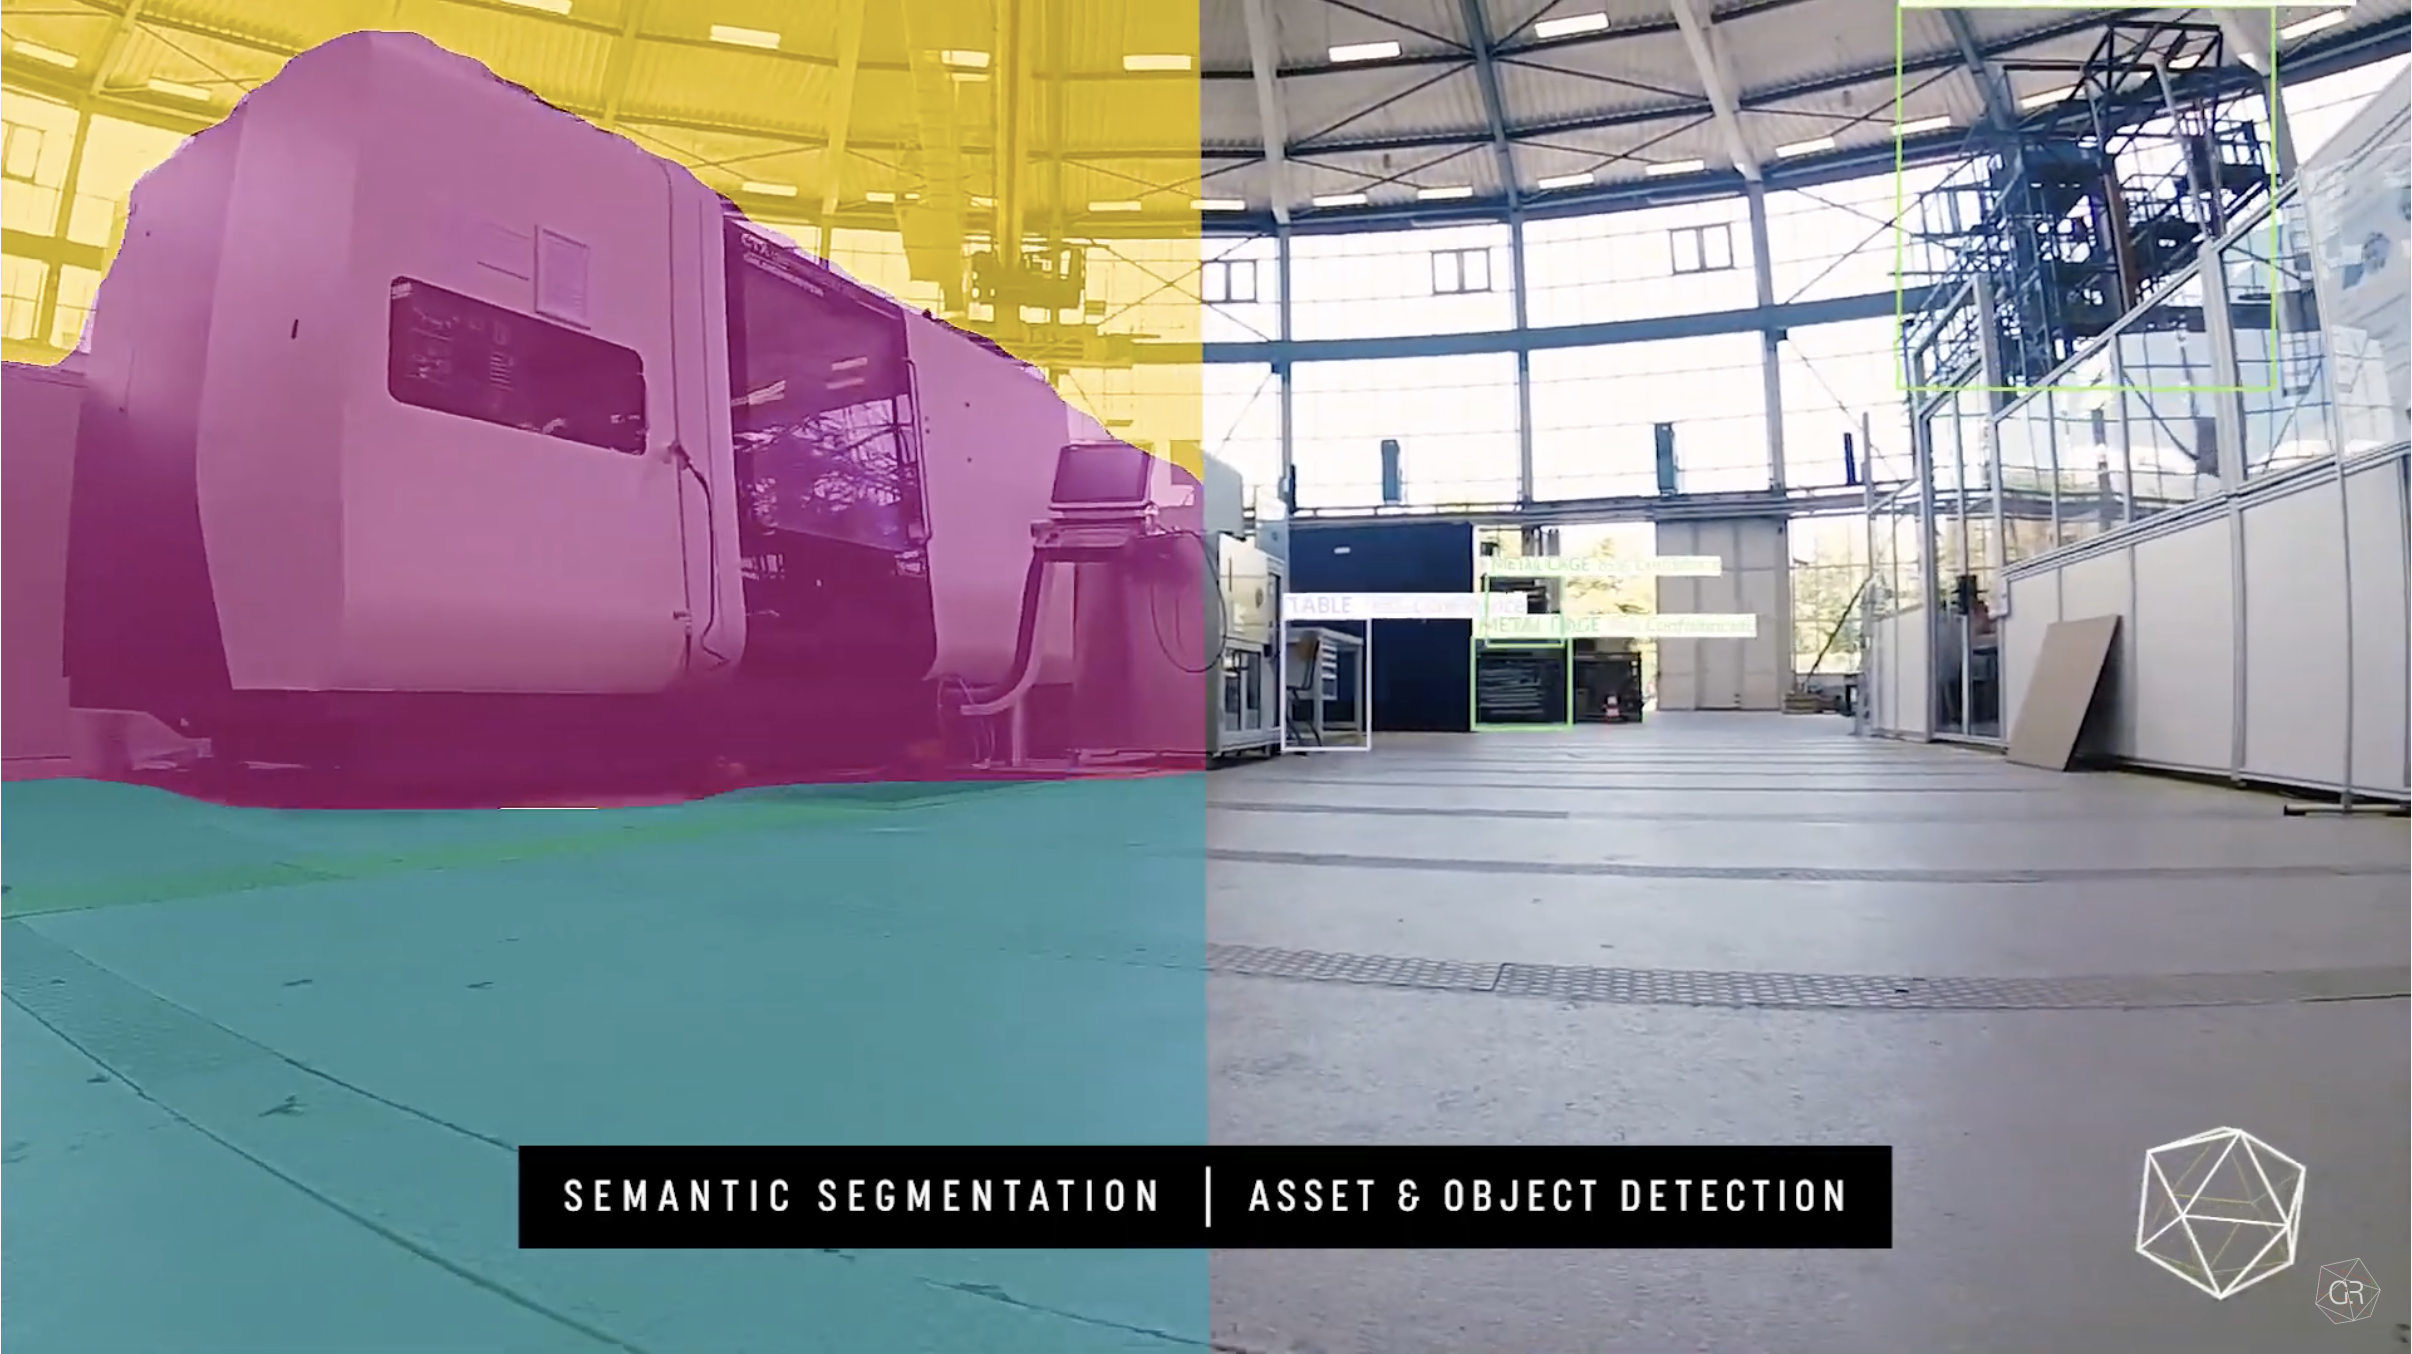
\includegraphics[scale=0.3]{SemanticSegmentation_ObjectDetection.png}
	\caption{Voorbeeld segmentatie + objectdetectie \autocite{Gestalt2019}}
\end{figure}

\subsubsection{Correctheid}
De 2de en meest cruciale factor is de correctheid van het AI-framework voor de verschillende soorten AI-eigenschappen. Het is belangrijk dat het framework betrouwbaar is en dus geen foute oplossing zal terug geven, anders zal dit verkeerd doorgegeven worden aan de visuele kant van de applicatie en zal de route verkeerd worden aangegeven. Om de correctheid van elk AI-framework te testen heeft men opnieuw de diverse AI-eigenschappen onder de loep genomen.

\subsubsection{Correctheid - 1.  Objectdetectie}
Om de objectdetectie te evalueren heeft men geobserveerd of het framework de juiste positie van het gerelateerde object aangeeft , alsook het percentage dat de correctie voorstelt werd in acht gehouden.

\subsubsection{Correctheid - 2. Menssegmentatie}
Bij de evaluatie van de menssegmentatie werd er gekeken of het computer gegenereerde oppervlak overeen kwam met de vorm van de daadwerkelijke persoon. De foute zones werden aangeduid met markeringen om een duidelijk overzicht te krijgen.

\subsubsection{Correctheid - 3. Luchtsegmentatie}
Luchtsegmentatie werd op dezelfde manier beoordeeld als menssegmentatie. Deze twee segmentaties hebben een zeer gelijkaardige input en output, maar toch is er een groot verschil binnenin het framework. Het algoritme wordt op een andere manier getraind en zo is er toch een mogelijkheid dat deze twee segmentaties voor verschillende resultaten zorgen.

\subsubsection{Correctheid - 4. Segmentatie binnen gebouwen}
Segmentatie binnen gebouwen is de uitwerking die het meest gerelateerd is met de AI-output die voor deze bachelorproef van belang is. Het biedt namelijk de mogelijkheid om muren van grond te onderscheiden, dit is de hoofdreden waarom men AI in deze wayfinding-uitwerking wilt betrekken. Het is dus belangrijk dat deze AI-uitwerking grondig wordt geëvalueerd.

De evaluatie verliep als volgt, voor beide AI-frameworks werd op identiek dezelfde plaats de test uitgevoerd. De resultaten werden naast elkaar geplaatst en vervolgens geëvalueerd door de foute zones aan te duiden, ook werd er gekeken naar de extra info die men kon vergaren uit beide resultaten. Het framework die het best de verschillende soorten segmenten kon 'vertellen', werd gezien als beste framework in deze sectie.

\begin{figure}[H]
	\centering
	\includegraphics[scale=0.3]{BeoordelingsTechnieken.png}
	\caption{Voorbeeld evaluatietechniek segmentatie binnen gebouwen}
\end{figure}

\subsubsection{Toegankelijkheid}
Een tweede belangrijke factor is de toegelankelijkheid van de AI-frameworks voor verschillende platformen. Zo is het belangrijk voor het bedrijf 'In The Pocket' dat ze een oplossing vinden dat schaalbaar is.

\subsection{Bepalen van optimaal AI-framework}
Het bepalen van welk AI-framework de optimale oplossing biedt werd gemaakt op basis van een overzicht van alle testen. Dit overzicht bevat staafdiagrammen die de resultaten van alle testen in kaart brengt, zo kan men rekening houden met de verschillende eigenschappen die elk framework te bieden heeft.

\chapter{\IfLanguageName{dutch}{Onderzoek}{Research}}
\label{ch:onderzoek}
In dit hoofdstuk zal de effectieve uitwerking van het onderzoek toegelicht worden. In het vorige hoofdstuk werd reeds het 'raamwerk' geschetst, dit hoofdstuk zal hier dus op verder gaan.In dit hoofdstuk zullen volgende zaken toegelicht worden:

\begin{itemize}
	\item Het bestuderen van de verschillende frameworks
	\item De AI-eigenschappen van elk framework valideren naargelang een vooropgestelde trainingset
	\item De resultaten bespreken voor elke AI-eigenschap
\end{itemize}

\section{De werking van de frameworks}
In deze sectie zullen de effectieve tests worden uitgevoerd, men zal steeds de resultaten van elk algoritme bespreken.

\subsection{Objectdetectie}

Zoals men eerder al heeft vermeld is objectdetectie een belangrijke factor binnen de wayfinding-context, men zal namelijk moeten weten waar elk object binnen een bepaalde kamer zich bevindt. Om dit op een goede manier te kunnen testen heeft men vijf verschillende objecten genomen en getest of men verschillende waarnemingen kon constateren. Om de resultaten te kunnen meten heeft men gebruik gemaakt van twee verschillende applicaties, 'Fritz AI Studio' en 'TFL Detect', beide applicaties werden uitgevoerd op een iPhone 11. Beide frameworks maakten immers gebruik van de COCO dataset.


\subsubsection{Tests}
	\begin{figure}[H]
		\centering
		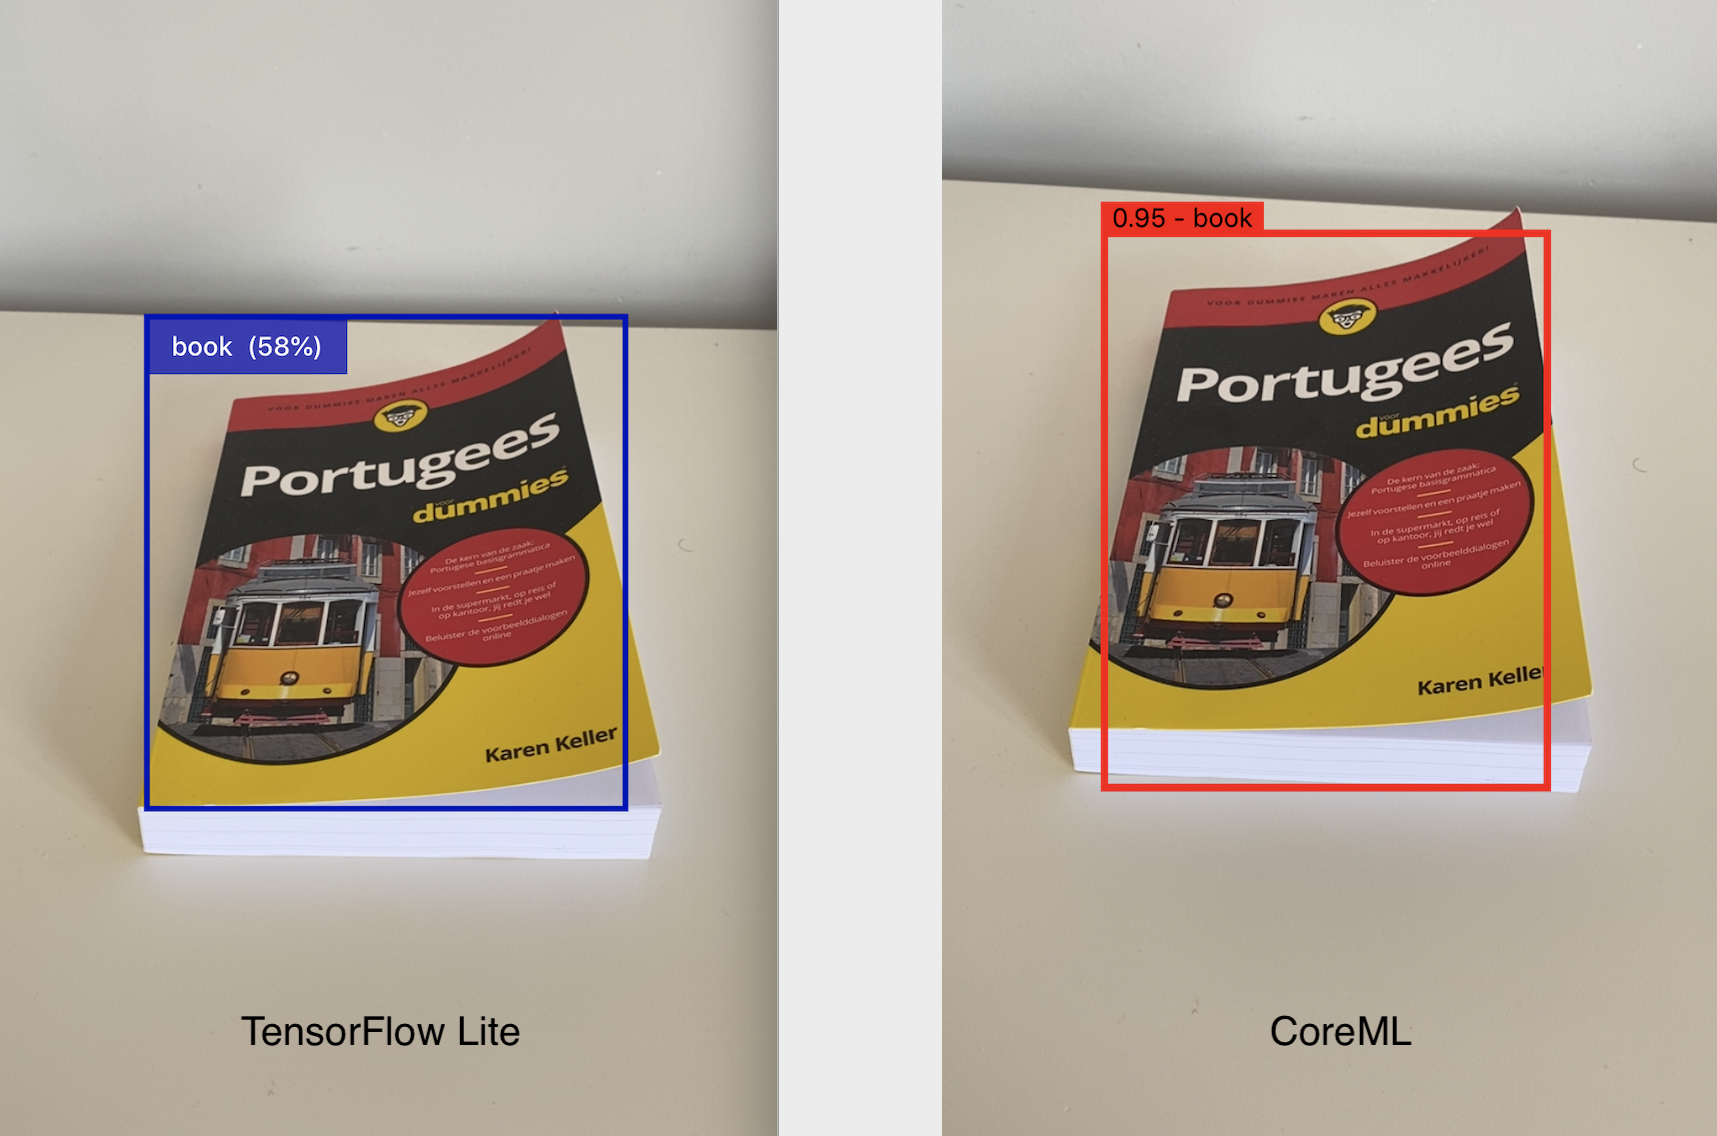
\includegraphics[scale=0.3]{ObjectDetection_Book.png}
		\caption{Test met boek, TensorFlow Lite (58\%) \& CoreML (95 \%)}
	\end{figure}
In de eerste objectdetectie-test kan men reeds waarnemen dat het boek beter wordt gedetecteerd door het CoreML-framework. Ten eerste wordt het boek nauwkeuriger aangeduid door de rechthoek, en ten tweede is het percentage veel beter. Het percentage dat de zekerheid aanduidt is namelijk 95 \% bij CoreML en 58 \% bij TensorFlow Lite.

\begin{figure}[H]
	\centering
	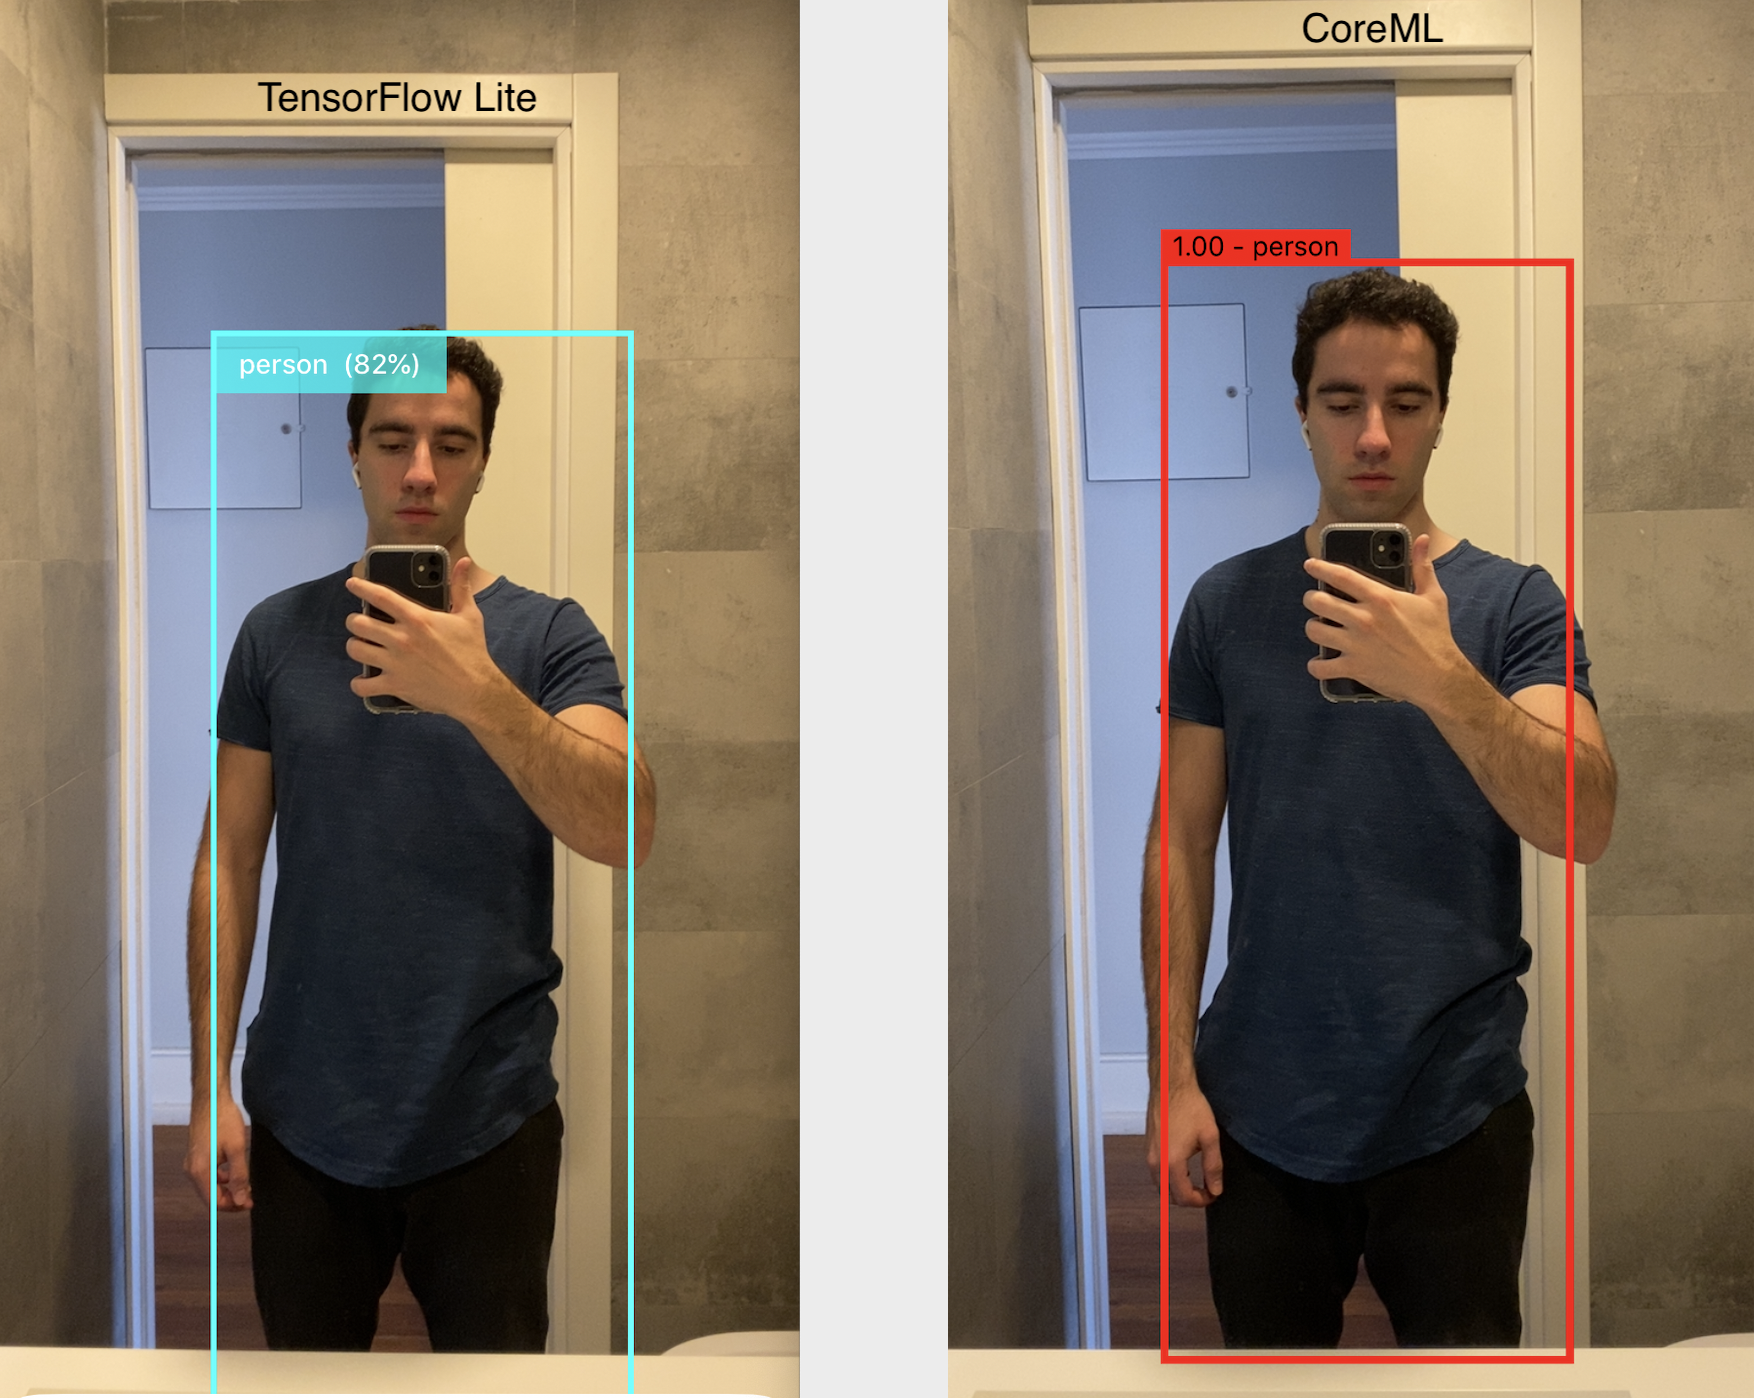
\includegraphics[scale=0.3]{ObjectDetection_Person.png}
	\caption{Test met persoon, TensorFlow Lite (82\%) \& CoreML (100 \%)}
\end{figure}
De tweede test toont nogmaals aan dat CoreML beter scoort. De persoon wordt veel exacter aangeduid met behulp van het vierkant. Het correctheidspercentage is nogmaals beter bij het CoreML-framework, men kan zelfs opmerken dat dit framework met 100\% kan zeggen dat het object een persoon is, dit resultaat is zeer opmerkelijk.

\begin{figure}[H]
	\centering
	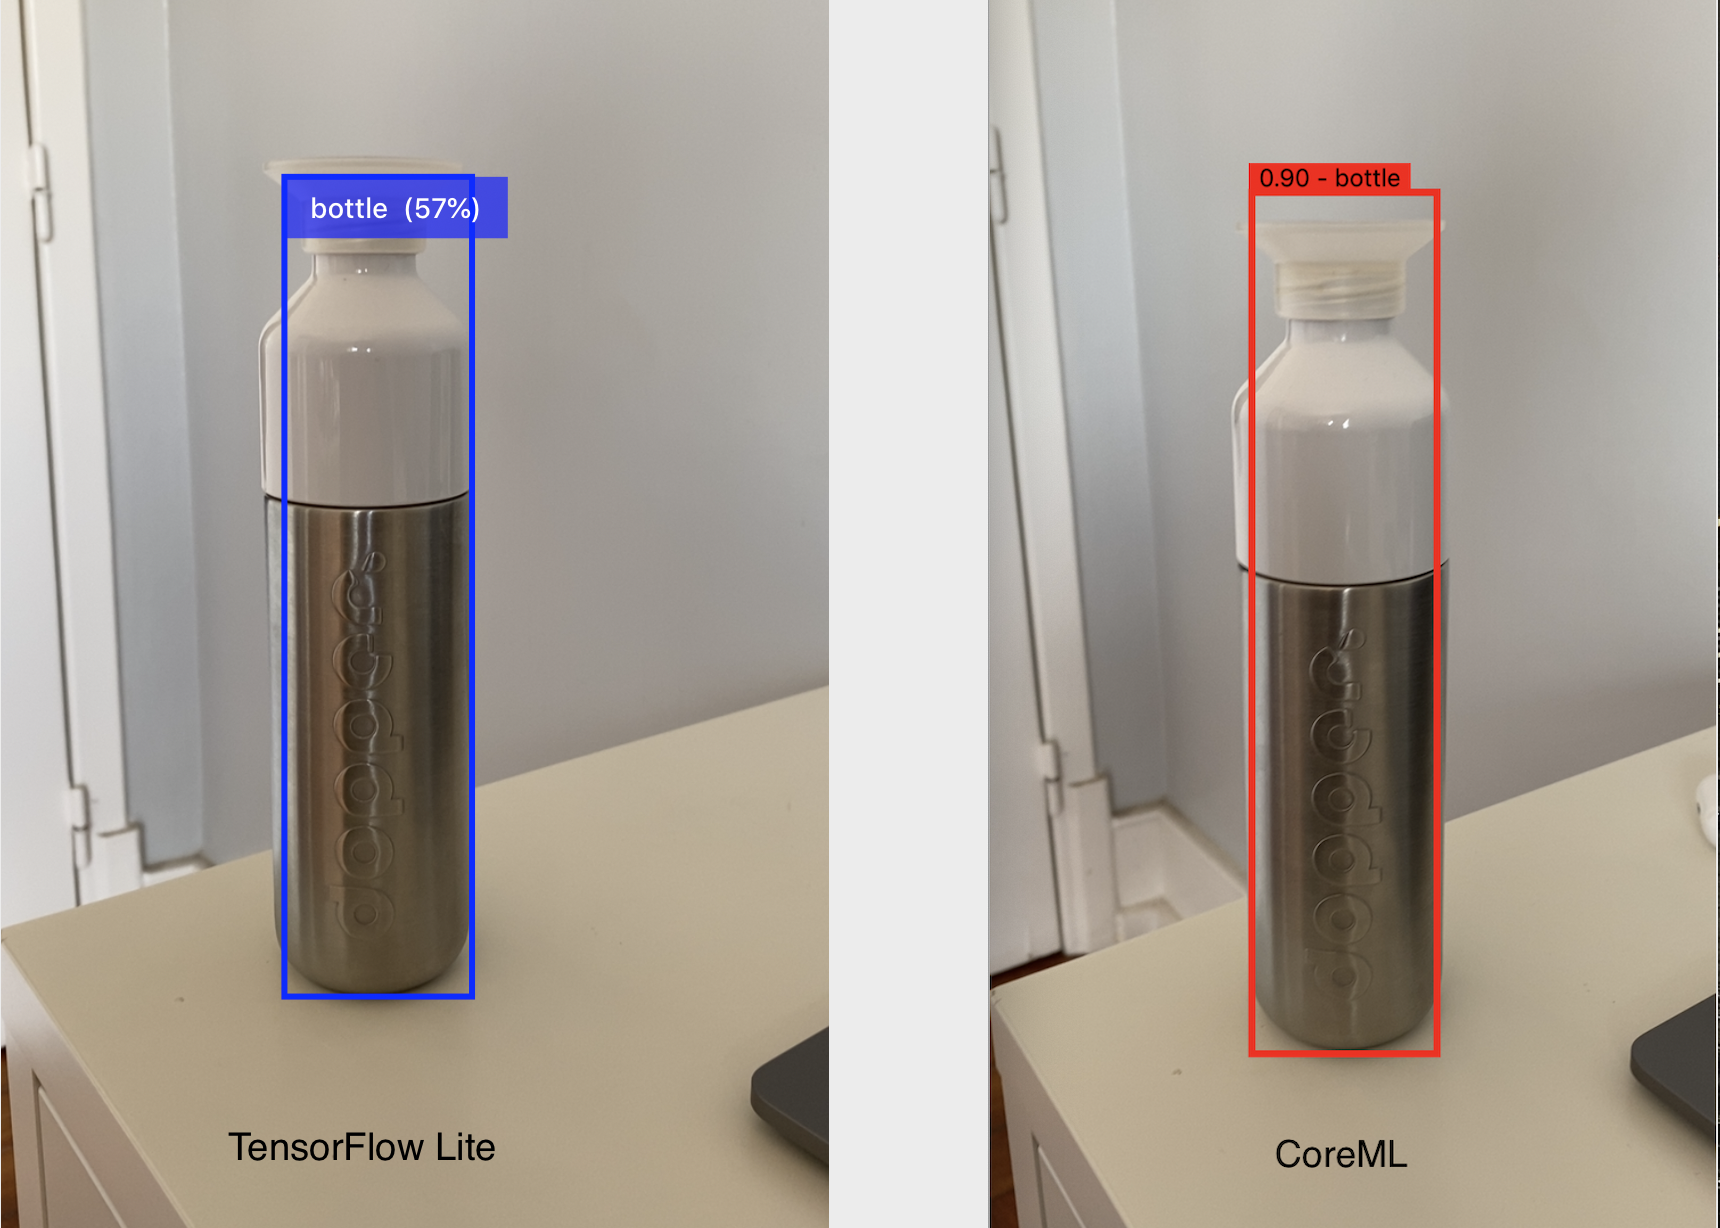
\includegraphics[scale=0.35]{ObjectDetection_Bottle.png}
	\caption{Test met waterfles, TensorFlow Lite (57\%) \& CoreML (90 \%)}
\end{figure}
Men kan opnieuw besluiten dat het framework van Apple een betere zaak doet om de waterfles te herkennen. Opnieuw kan men een significant correctheidsverschil opmerken tussen beide frameworks. CoreML kan in dit geval men bijna 30 \% meer zekerheid zeggen dat het vertoonde object een fles is.
\begin{figure}[H]
	\centering
	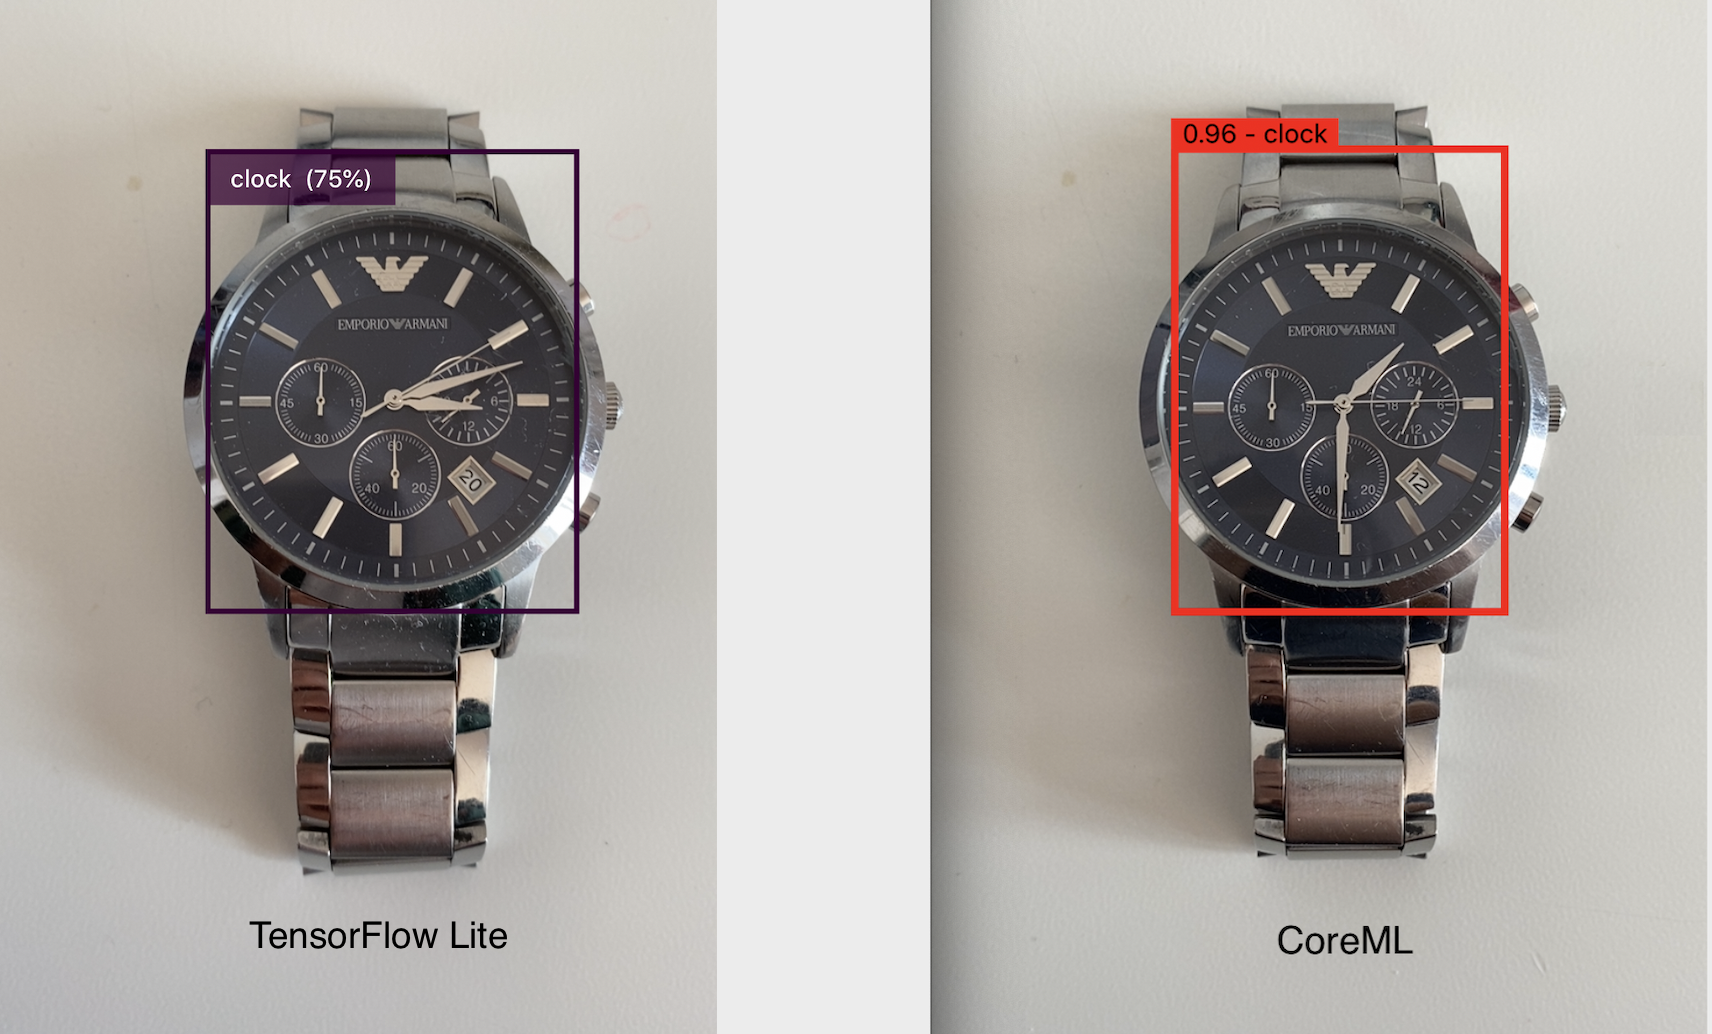
\includegraphics[scale=0.38]{ObjectDetection_Clock.png}
	\caption{Test met horloge, TensorFlow Lite (75 \%) \& CoreML (96 \%)}
\end{figure}
Andermaal kan men waarnemen dat het CoreML-framework betere resultaten levert als TensorFlow Lite, men kan in dit geval wel opmerken dat de detectie a.d.h.v het vierkant nauwkeuriger werd uitgevoerd door het TensorFlow Lite-framework. Opnieuw kan men een nauwkeurigheidsverschil opmerken van meer dan 20 \%.

\begin{figure}[H]
	\centering
	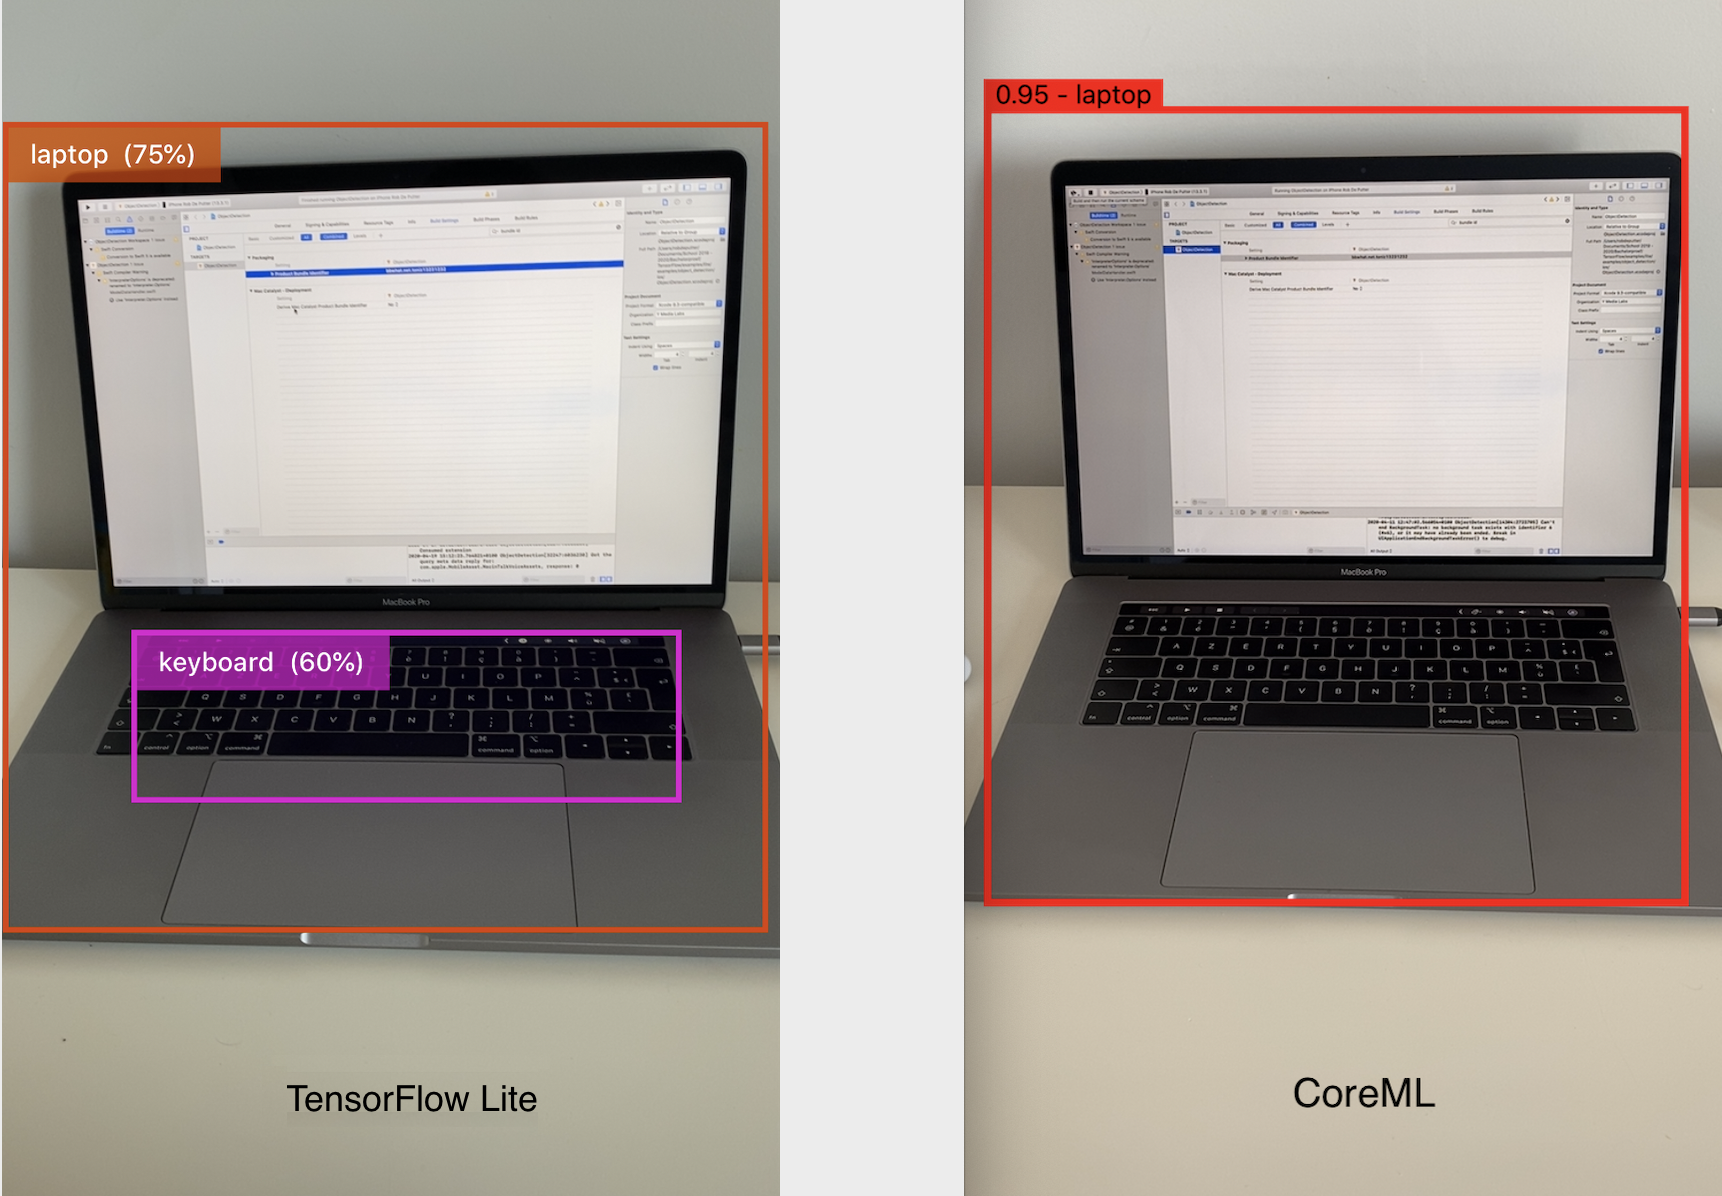
\includegraphics[scale=0.38]{ObjectDetection_Laptop.png}
	\caption{Test met laptop, TensorFlow Lite (75 \%) \& CoreML (95 \%)}
\end{figure}
De laatste test verschilt van de anderen, men kan namelijk bemerken dat TensorFlow Lite het toestenbord kan bespeuren, terwijl CoreML niet in staat is om dit te doen. De nauwkeurigheid kent wel lagere cijfers, opnieuw is er een verschil van 20 \% op vlak van accuraatheid.
	
\subsubsection{Evaluatie}
Men kan concluderen dat CoreML veel beter in staat is om de verschillende objecten te detecteren en vervolgens ook te herkennen. De verschillen tussen de beide frameworks is opmerkelijk, zeker als men weet dat ze beiden werden getraind met dezelfde dataset. Het eindresultaat uit deze testen zal met zekerheid een beslissingsfactor zijn voor het maken van de eindbeslissing.

\subsection{Menssegmentatie}
De tweede AI-eigenschap die men getest heeft is menssegmentatie, in deze eigenschap zal men de volledige foto gaan onderzoeken of er zich mensen in begeven. Indien er zich mensen in het beeld bevinden zal het algoritme deze aanduiden door een bepaald kleuroppervlak over deze objecten te plaatsen. De resultaten werden bekomen door gebruik te maken van de 'Fritz AI Studio' applicatie op twee verschillende apparaten, namelijk een iPhone 11 (iOS) en een Huawei P Smart 2019 (Android). In de documentatie van de 'Fritz AI Studio' applicatie kan men opmerken dat de Android-variant gebruik maakt van TensorFlow Lite en de iOS-variant CoreML utiliseert. Deze beide frameworks gebruiken hetzelfde voorgetrainde model, dit werd samengesteld door Fritz AI.

\subsubsection{Test}

\begin{figure}[H]
	\centering
	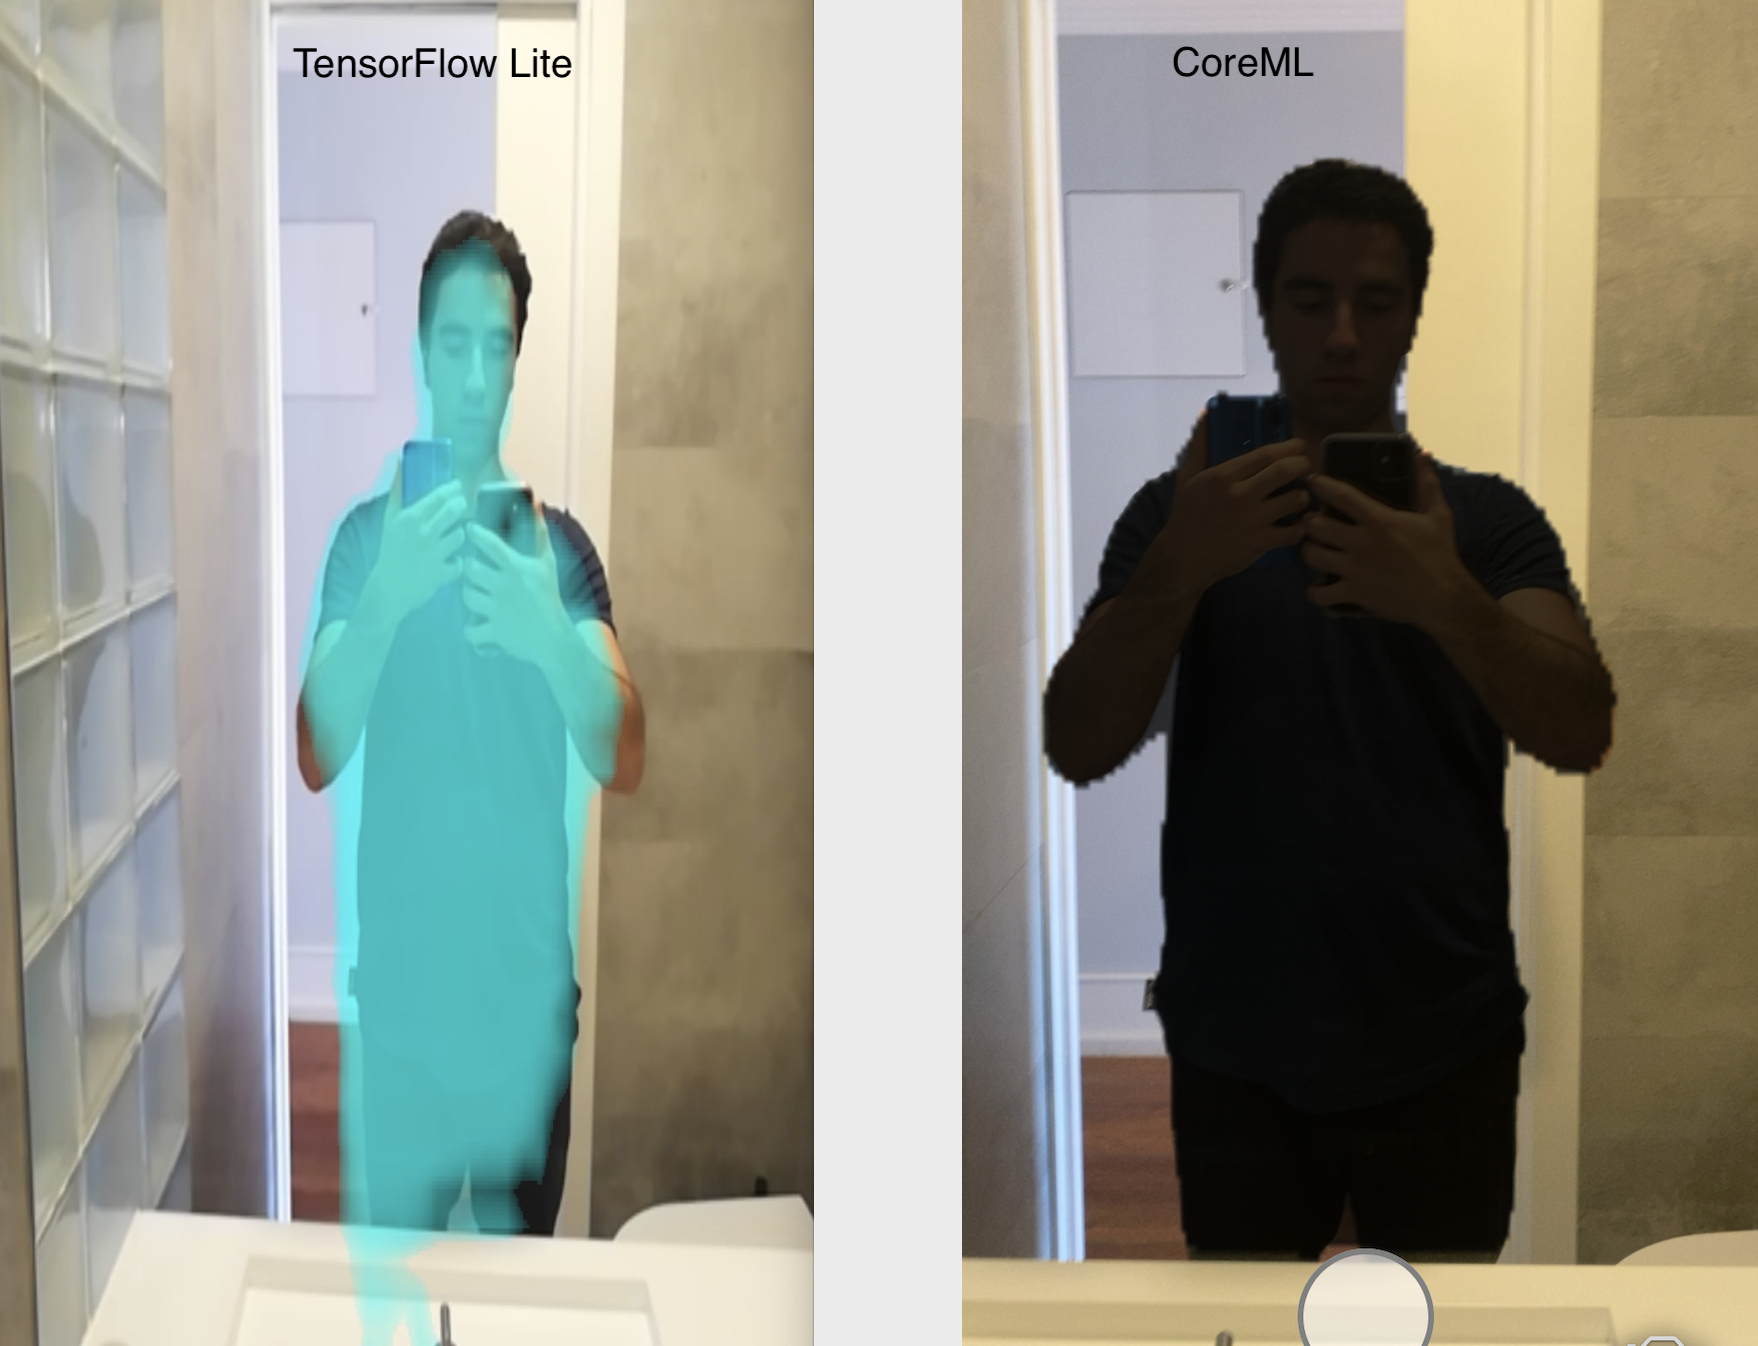
\includegraphics[scale=0.3]{PeopleSegmentation.png}
	\caption{Test menssegmentatie, zonder foutaanduiding}
\end{figure}
Uit de resultaten van deze test kan men opnieuw aanschouwen dat het CoreML-framework een veel betere uitslag levert dan TensorFlow Lite. Ondanks dezelfde dataset slaagt CoreML er toch in om de persoon in de afbeelding bijna 100 \% correct aan te duiden, de uitkomst van het andere framework is niet nauwkeurig en kent zelfs grove fouten. Men kan concluderen dat het CoreML-framework veel nauwkeuriger is. In de onderstaande afbeelding kan men de foute zones waarnemen, de rode vlaktes tonen aan waar de persoon niet werd gedetecteerd, maar wel was. Het gele gebied duidt de zones aan waar de persoon werd gedetecteerd, maar niet was.

\begin{figure}[H]
	\centering
	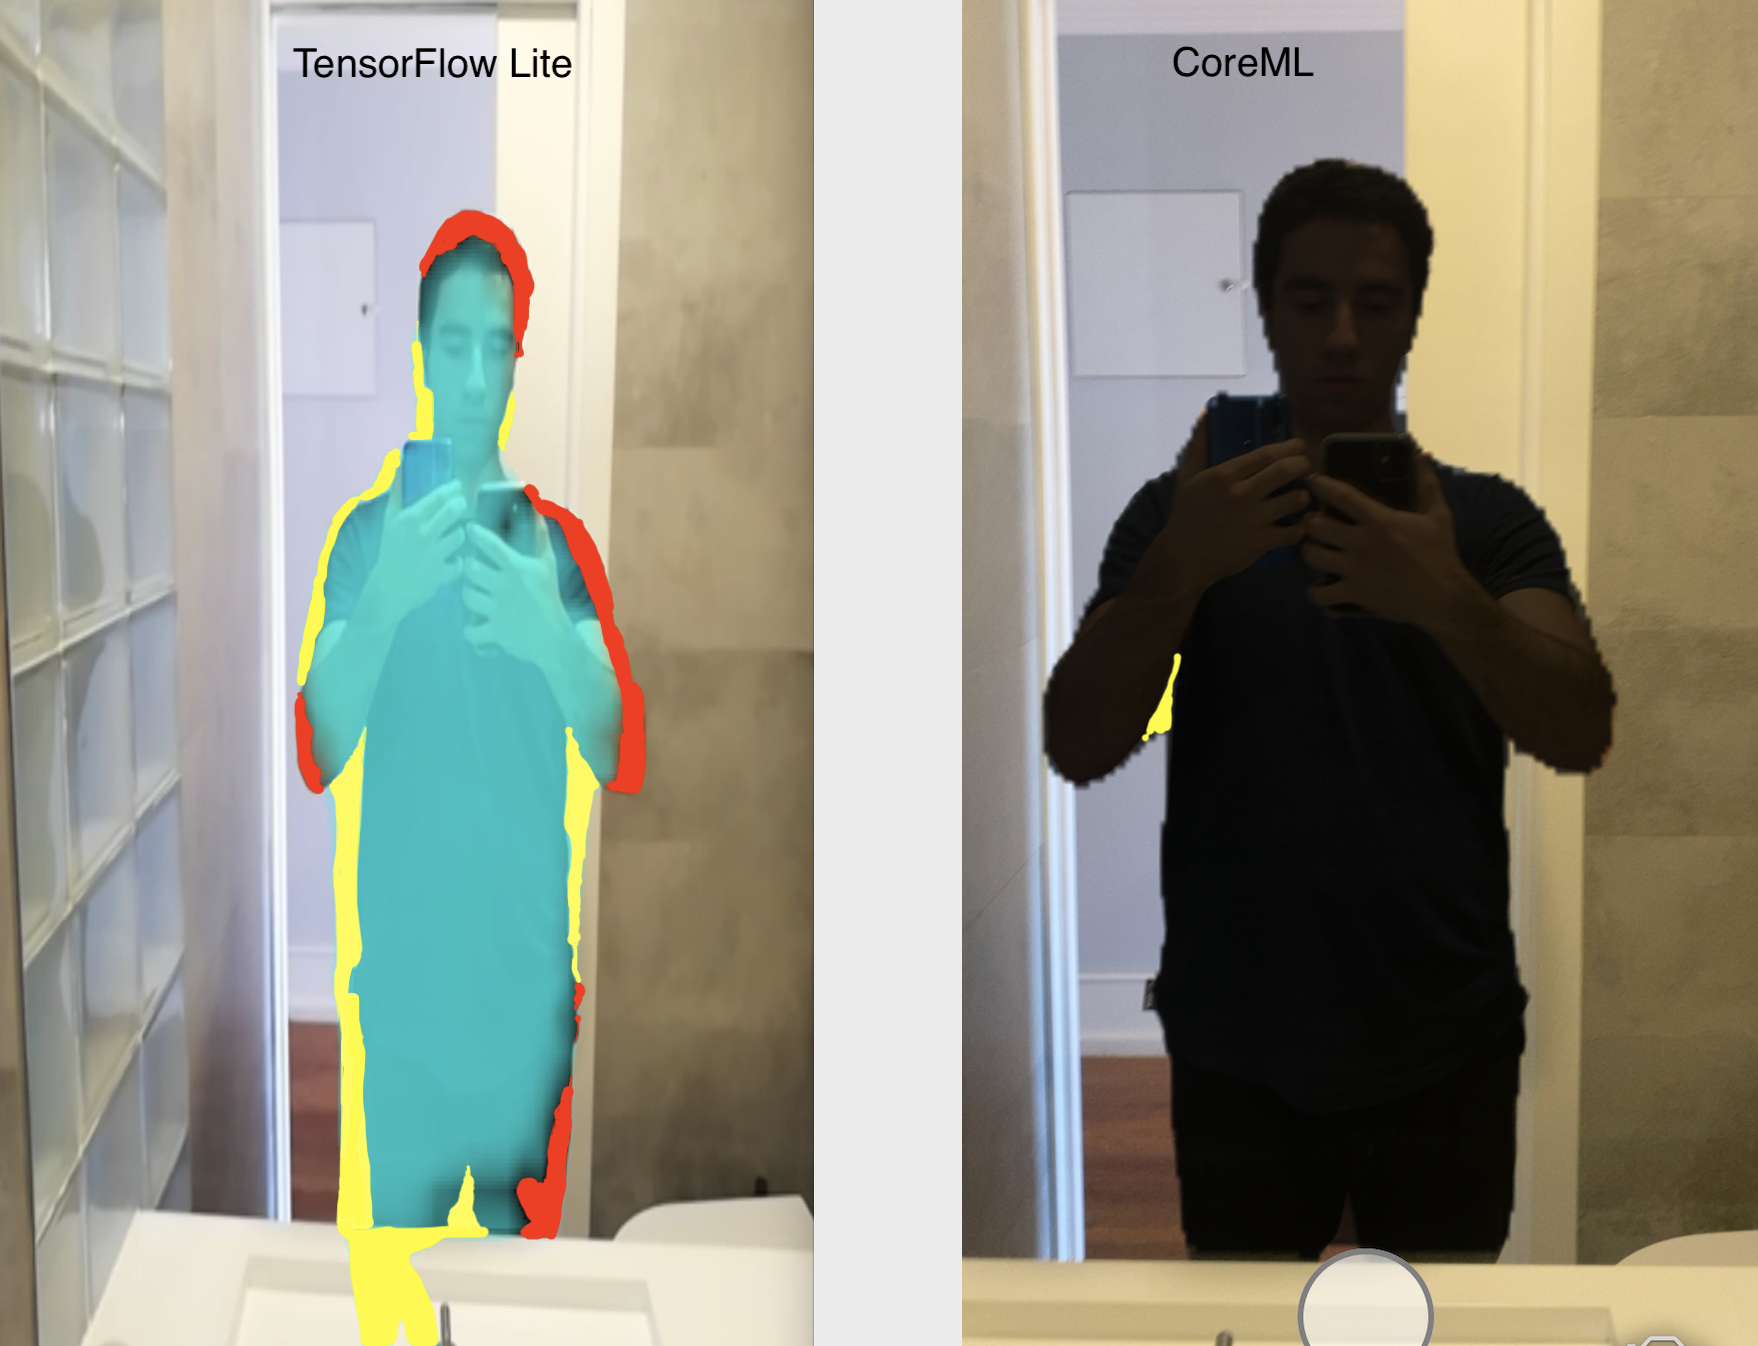
\includegraphics[scale=0.3]{PeopleSegmentation_MetFoutAanduiding.png}
	\caption{Test menssegmentatie, met foutaanduiding}
\end{figure}
\subsubsection{Evaluatie}
De link tussen menssegmentatie en de wayfinding-context kan misschien ver te zoeken zijn, maar deze test zegt wel degelijk meer over de precisie van het AI-framework. Alsook is het mogelijk dat een groep mensen de weg kan versperren, in dit geval is het belangrijk dat deze groep wordt gedetecteerd door het algoritme, een zekere mensherkenning en detectie is dus zeker van belang.

Uit de resultaten van deze test kan men dus opnieuw concluderen dat het CoreML-framework een betere keuze is op het vlak van precisie en correctheid.
\subsection{Luchtsegmentatie}
\subsubsection{Test}

\subsubsection{Evaluatie}

\subsection{Segmentatie binnen gebouwen}
\subsubsection{Test}

\subsubsection{Evaluatie}

\chapter{\IfLanguageName{dutch}{Resultaten}{Results}}
\label{ch:resultaten}

